\section{Model Selection Study}
\label{sec:models}
The first stage of the cascade is LightGBM, and this section tests that choice. The study ran in three stages. Two earlier stages on other datasets compared classical machine learning with deep learning, and a wider stage surveyed about 50 classical models on the same two datasets. A new comparison on Edge-IIoTset then used the split, features and metric of the rest of this paper. The earlier stages are public repositories of the same project; every number below is read from their result files.

\subsection{Earlier stages on MQTTset and DataSense}
Stage~1 compared eight supervised classifiers on MQTTset~\cite{vaccari2020}: random forest, logistic regression, gradient boosting, k-nearest neighbours, naive Bayes, an MLP, a 1D-CNN and a GRU, plus a one-class autoencoder trained on benign traffic. An RBF SVM, an LSTM and a vanilla RNN were added to the table. Stage~2 repeated the method on DataSense~\cite{firouzi2025}, the 2025 sensor-based IIoT benchmark from the Canadian Institute for Cybersecurity. Table~\ref{tab:prior} lists the results. Neither dataset gave a clear winner between the two families. On MQTTset, k-nearest neighbours had the highest macro F1 (0.819), ahead of the MLP (0.777), the GRU (0.768) and gradient boosting (0.724). On DataSense, the MLP (0.895) and gradient boosting (0.893) were level and the random forest followed at 0.884. The recurrent networks without sequence input were poor on both (LSTM 0.243 and vanilla RNN 0.095 macro F1 on DataSense). When the same CNN and GRU were retrained on windows of eight packets per flow, accuracy on MQTTset rose to 0.999, but that test measures a different task on a different sample and we do not compare it with the flat-feature models.

\begin{table}[t]
\centering
\caption{Earlier stages: classical and neural classifiers on MQTTset and DataSense, ordered by macro F1 within each dataset. MQTTset: 231,646 training and 99,290 test rows, 33 features. DataSense: 31,538 training and 13,517 test rows, 109 features. $^\dagger$ trained on a 40,000-row subsample because the full fit did not finish.}
\label{tab:prior}
\small
\begin{adjustbox}{max width=\linewidth}
\begin{tabular}{lccc}
\toprule
Model & Accuracy & Macro F1 & Train (s) \\
\midrule
\textit{MQTTset} & & & \\
\quad K-Nearest Neighbors & 0.9136 & 0.8188 & 0.0 \\
\quad MLP & 0.8513 & 0.7768 & 42.8 \\
\quad GRU & 0.8496 & 0.7681 & 122.7 \\
\quad Gradient Boosting & 0.8883 & 0.7235 & 4.4 \\
\quad Random Forest & 0.8856 & 0.7157 & 1.6 \\
\quad LSTM & 0.8286 & 0.6560 & 276.8 \\
\quad Logistic Regression & 0.6520 & 0.6305 & 9.7 \\
\quad 1D-CNN & 0.7312 & 0.6207 & 99.9 \\
\quad SVM (RBF)$^\dagger$ & 0.6467 & 0.5679 & 23.4 \\
\quad RNN & 0.8202 & 0.5038 & 212.9 \\
\quad Naive Bayes & 0.7946 & 0.4759 & 0.1 \\
\textit{DataSense} & & & \\
\quad MLP & 0.9448 & 0.8948 & 63.9 \\
\quad Gradient Boosting & 0.9516 & 0.8931 & 7.0 \\
\quad Random Forest & 0.9418 & 0.8842 & 0.8 \\
\quad 1D-CNN & 0.9244 & 0.8596 & 39.8 \\
\quad K-Nearest Neighbors & 0.9129 & 0.8452 & 0.0 \\
\quad SVM (RBF) & 0.8841 & 0.7667 & 22.2 \\
\quad GRU & 0.8672 & 0.7470 & 126.5 \\
\quad Logistic Regression & 0.8568 & 0.7357 & 1.3 \\
\quad Naive Bayes & 0.4655 & 0.4344 & 0.0 \\
\quad LSTM & 0.6228 & 0.2434 & 94.4 \\
\quad RNN & 0.6072 & 0.0945 & 103.0 \\
\bottomrule
\end{tabular}
\end{adjustbox}

\end{table}

Stage~3 widened the classical side. It trained about 50 scikit-learn-compatible classifiers on both datasets, covering linear models, naive Bayes, single trees, bagged trees, boosting (XGBoost, LightGBM, CatBoost, HistGradientBoosting and others), kernel and instance-based learners, interpretable models and ensembles. It ranked them by a composite of quality (macro F1, weighted F1 and F1 on the rarest class) and cost (inference time and training time), with weights of 0.7 for quality and 0.3 for cost. Stage~3 reuses the split of the first two stages (a model in both gives the same macro F1; k-nearest neighbours with $k=5$ scores 0.8188 on MQTTset in both), but it sub-sampled some slow models. Table~\ref{tab:top} lists the ten highest composite scores. Gradient-boosting implementations take the first five places, XGBoost first, with LightGBM fourth. This ranking is the reason boosting went forward. It has two limits: the cost weights were our own choice, and both datasets are far smaller and simpler than Edge-IIoTset.

\begin{table}[t]
\centering
\caption{Stage~3: ten best of 50 classical models by average composite score over MQTTset and DataSense (quality weight 0.7, cost weight 0.3).}
\label{tab:top}
\small
\begin{adjustbox}{max width=\linewidth}
\begin{tabular}{llccc}
\toprule
Model & Family & F1 MQTTset & F1 DataSense & Composite \\
\midrule
XGBoost (DART) & boosting & 0.8371 & 0.9618 & 99.9 \\
XGBoost & boosting & 0.8371 & 0.9618 & 99.9 \\
Hist Gradient Boosting & boosting & 0.8350 & 0.9585 & 99.5 \\
LightGBM & boosting & 0.8370 & 0.9614 & 99.5 \\
CatBoost & boosting & 0.8339 & 0.9523 & 99.2 \\
Gradient Boosting (sklearn) & boosting & 0.8334 & 0.9553 & 96.5 \\
K-Nearest Neighbors (k=15, distance-weighted) & instance & 0.8274 & 0.8487 & 92.4 \\
Explainable Boosting Machine & interpretable & 0.8284 & 0.9555 & 91.9 \\
K-Nearest Neighbors (k=5) & instance & 0.8188 & 0.8452 & 91.8 \\
Voting Classifier (soft) & meta & 0.7618 & 0.9210 & 90.5 \\
\bottomrule
\end{tabular}
\end{adjustbox}

\end{table}

\subsection{Comparison on Edge-IIoTset}
\label{sec:zoo}
\textit{Protocol.} The new comparison uses the 130-feature matrix and the connection-grouped split of Section~\ref{sec:featstudy} (seed 42): 397,073 test rows, none from a connection seen in training. Every model trains on the same class-capped stratified sample of 500,000 training rows, because slow learners cannot be run on all 1.43 million, and is scored on the full test split. Hyperparameters were chosen on a separate validation sample of 60,000 rows and never on the test rows. Each model had a small grid (for example tree depth, number of leaves, regularisation strength or $k$); the grid and the chosen value are stored with the results. Models that accept class weights use the same square-root weights as the system, and the neural networks use them in the loss. The RBF SVM was trained on a 40,000-row subsample and the GRU on 150,000 rows, for the same feasibility reason. Metrics are accuracy, macro F1 over the classes present in the test split, benign false-positive rate, training time on 16 CPU threads and prediction time per row.

\begin{table*}[t]
\centering
\caption{Edge-IIoTset, 130 features, connection-grouped test split (397,073 rows, seed 42): 15 classifiers trained on the same 500,000-row sample, ordered by macro F1. Train and predict times are wall-clock on 16 CPU threads, one job at a time. Values marked $^\ddagger$ come from a separate run of that model alone on the machine.}
\label{tab:zoo}
\small
\begin{adjustbox}{max width=\linewidth}
\begin{tabular}{llccccrr}
\toprule
Model & Family & Acc. & Macro F1 & Weighted F1 & Benign FPR & Train (s) & Predict ($\mu$s/row) \\
\midrule
Random forest & bagging trees & 0.9970 & 0.9848 & 0.9970 & 0.0010 & 13 & 3.8 \\
HistGradientBoosting & boosting & 0.9970 & 0.9838 & 0.9970 & 0.0012 & 39$^\ddagger$ & 15.5$^\ddagger$ \\
XGBoost & boosting & 0.9971 & 0.9834 & 0.9972 & 0.0010 & 30 & 1.2 \\
Decision tree & single tree & 0.9967 & 0.9828 & 0.9968 & 0.0010 & 7 & 0.1 \\
CatBoost & boosting & 0.9970 & 0.9813 & 0.9970 & 0.0011 & 315 & 0.7 \\
LightGBM & boosting & 0.9971 & 0.9805 & 0.9971 & 0.0010 & 8 & 1.3 \\
Extra trees & bagging trees & 0.9968 & 0.9792 & 0.9968 & 0.0010 & 19 & 3.8 \\
k-nearest neighbours & instance & 0.9956 & 0.9706 & 0.9956 & 0.0012 & 0$^\ddagger$ & 261.3$^\ddagger$ \\
1D-CNN & neural & 0.9953 & 0.9640 & 0.9954 & 0.0016 & 96$^\ddagger$ & 17.6$^\ddagger$ \\
MLP & neural & 0.9959 & 0.9631 & 0.9959 & 0.0015 & 18$^\ddagger$ & 0.2$^\ddagger$ \\
Logistic regression & linear & 0.9937 & 0.9314 & 0.9941 & 0.0016 & 56 & 0.1 \\
GRU (150k train rows) & neural & 0.9857 & 0.9253 & 0.9856 & 0.0038 & 388 & 21.1 \\
RBF SVM (40k train rows) & kernel & 0.9901 & 0.9217 & 0.9905 & 0.0039 & 19$^\ddagger$ & 837.8$^\ddagger$ \\
Linear SVM & linear & 0.9912 & 0.9093 & 0.9925 & 0.0017 & 7 & 0.1 \\
Gaussian naive Bayes & probabilistic & 0.5258 & 0.7115 & 0.6456 & 0.5886 & 0 & 4.4 \\
\bottomrule
\end{tabular}
\end{adjustbox}

\end{table*}

\begin{figure}[t]
\centering
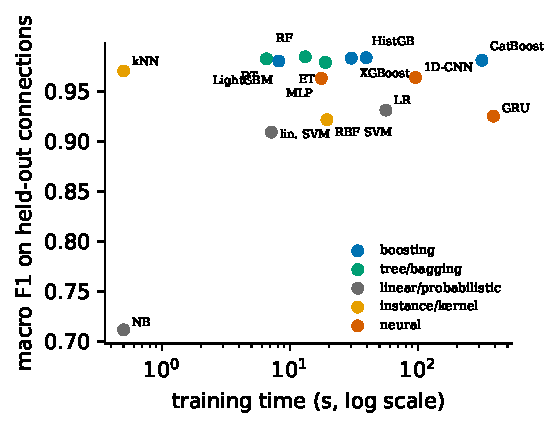
\includegraphics[width=\columnwidth]{figs/fig_zoo.pdf}
\caption{Macro F1 against training time for the 15 classifiers of Table~\ref{tab:zoo}.}
\label{fig:zoo}
\end{figure}

\textit{Results.} Seven tree-based models fill the top of Table~\ref{tab:zoo}, with macro F1 between 0.979 and 0.985: random forest 0.985, HistGradientBoosting 0.984, XGBoost 0.983, a single decision tree 0.983, CatBoost 0.981, LightGBM 0.981 and extra trees 0.979. The spread of 0.006 is the same size as the seed-to-seed spread of one model, since LightGBM on the full training set scores 0.983, 0.984 and 0.985 across the three seeds of Table~\ref{tab:seeds}. We therefore do not rank these seven. k-nearest neighbours follows at 0.971, the 1D-CNN and the MLP at 0.964 and 0.963, logistic regression at 0.931, the RBF SVM on 40,000 rows at 0.922 and the linear SVM at 0.909. Gaussian naive Bayes collapses (0.712, with 59\% of benign rows flagged); it was also among the weakest models in the earlier stages. The GRU, which reads the 130 features as a sequence of 130 steps, reached 0.925 after 20 epochs on 150,000 rows. A first 3-epoch run scored only 0.106, and the 20-epoch validation score was still rising, so we treat the GRU as under-trained and its score as no final value for that architecture. The benign false-positive rate is 0.10 to 0.12\% for every tree model and rises to 0.15 to 0.16\% for the neural networks and logistic regression.

On this feature set the choice among tree models hardly matters: a single decision tree of depth 20 is within 0.002 of the best. That fits the feature study of Section~\ref{sec:featstudy}. Once the connection features make the classes separable (the ambiguity ceiling is 0.9997 macro recall), the model has little left to add. The trees do beat the neural networks, by about 0.02 macro F1, and the linear models by 0.05 or more. Cost separates the families less than accuracy does. The trees train in 7 to 39~s (CatBoost 315~s), the MLP in 18~s, the 1D-CNN in 96~s and the GRU in 388~s. A prediction takes 0.1 to 16~$\mu$s per row for every tree model, 0.2 to 26~$\mu$s for the networks, and 261 and 838~$\mu$s for the two instance-based and kernel models.

\subsection{Boosting on the base features}
\label{sec:basezoo}
The earlier head-to-head of LightGBM and an MLP used the 91 base features and showed a large gap, 0.887 against 0.622 macro F1 on a 500,000-row class-capped sample (Table~\ref{tab:mlp}). The gap was largest on the application-layer attacks that the base features cannot separate. To see how much of it comes from the features rather than the learners, we repeated the comparison above with the 91 base features. Nine of the 15 models were run (the other six were not repeated); Table~\ref{tab:zoobase} gives the results. On the base features the boosting implementations lead clearly: XGBoost 0.875, LightGBM 0.854 and CatBoost 0.852, against 0.807 for the random forest, 0.788 for extra trees and 0.777 for a single decision tree. The MLP (0.596), k-nearest neighbours (0.560) and logistic regression (0.402) are far behind. The MLP's score is close to the 0.622 of the earlier head-to-head, which used a different sample. Adding the 39 service-port, content and connection features raises every model, from $+0.11$ for XGBoost to $+0.53$ for logistic regression, and it closes the gap between boosting and the bagged trees: random forest gains $+0.18$ and reaches the top of Table~\ref{tab:zoo}. The two feature sets give different test rows (381,742 and 397,073, because deduplication differs), so the differences are approximate.

\begin{table}[t]
\centering
\caption{Nine classifiers on the 91 base features and on the 130 features (connection-grouped split, seed 42; 500,000 training rows). The last column is the macro-F1 gain from the 39 added features.}
\label{tab:zoobase}
\small
\begin{adjustbox}{max width=\linewidth}
\begin{tabular}{lcccc}
\toprule
Model & Acc.\ (91) & Macro F1 (91) & Macro F1 (130) & Gain \\
\midrule
XGBoost & 0.9416 & 0.8748 & 0.9834 & +0.1086 \\
LightGBM & 0.9330 & 0.8541 & 0.9805 & +0.1264 \\
CatBoost & 0.9311 & 0.8519 & 0.9813 & +0.1294 \\
Random forest & 0.9104 & 0.8068 & 0.9848 & +0.1780 \\
Extra trees & 0.9056 & 0.7877 & 0.9792 & +0.1914 \\
Decision tree & 0.8912 & 0.7774 & 0.9828 & +0.2054 \\
MLP & 0.8240 & 0.5956 & 0.9631 & +0.3675 \\
k-nearest neighbours & 0.7349 & 0.5603 & 0.9706 & +0.4103 \\
Logistic regression & 0.4781 & 0.4018 & 0.9314 & +0.5296 \\
\bottomrule
\end{tabular}
\end{adjustbox}

\end{table}

So the earlier result and the new one agree. Boosting is the best choice when the features are weak, and its edge over bagged trees disappears when the features are strong.

\begin{table}[t]
\centering
\caption{LightGBM against a dense MLP on the 91 base features, 500,000-row class-capped sample (400,000 training and 100,000 test rows, random split; Normal is about 10\% of the sample). The MLP has hidden layers of 64 and 32 units, dropout 0.1 and 8,271 parameters, trained for 15 epochs.}
\label{tab:mlp}
\small
\begin{tabular}{lcc}
\toprule
 & LightGBM & MLP \\
\midrule
Accuracy & 0.8908 & 0.6779 \\
Macro F1 & 0.8872 & 0.6218 \\
Weighted F1 & 0.8924 & 0.6681 \\
Benign FPR & 0.1599 & 0.5341 \\
Training time (s) & 55.5 & 10.2 \\
Model size & 12.8 MB (300 rounds) & 8,271 parameters \\
\bottomrule
\end{tabular}
\end{table}

In that comparison the gap is largest on XSS (recall 0.761 against 0.072), SQL\_injection (0.767 against 0.213), Fingerprinting (0.579 against 0.000), Port\_Scanning (0.997 against 0.499) and Uploading (0.630 against 0.198), and near zero on the three DDoS floods, which both models classify almost perfectly. The MLP is slightly better on Password and DDoS\_ICMP. The comparison is limited: the MLP is small and was not tuned, the sample uses the unrepaired MITM rows, and its class mix makes the false-alarm rates incomparable with the rest of the paper.

\subsection{Why LightGBM}
Three results favour boosting and one does not. Boosting implementations took the first five places among 50 classical models on two other datasets (stage~3), and on the 91 base features LightGBM beat the MLP by 0.27 macro F1. On the 130 features LightGBM sits inside the top group of tree models, trains in 8~s and produces a model of 9 to 10~MB. It also supports continued training from an existing model, which the incremental update of Section~\ref{sec:booster} needs. What the study does not show is that boosting is the best first stage on the 130 features: random forest, HistGradientBoosting, XGBoost and a single decision tree scored as high or higher in this run. We kept LightGBM because the system was built and evaluated around it before this comparison was run.
